% stuff on second day


\begin{frame}
    \only<1-3>{\begin{align*}
            \frac{\mathbf{U}}{\mathbf{R}} &\stackrel{!}{=} \mathbf{I} = \frac{\mathbf{U}}{R}& 
            \mathllap{\mathbf{I} \coloneqq \hat{I} \cdot e^{\mathbf{i}\omega t}} \\[1.4em]
            \visible<2-3>{
                \implies \mathbf{R} &= \frac{R \cdot \mathbf{I}}{\mathbf{I}} 
                \visible<3>{
                    = R \qquad \\[0.6em]
                    \mathbf{I} &= \frac{\hat{U}}{\mathbf{R}} \cdot e^{\mathbf{i}\omega t}
                }
            }
    \end{align*}}
    \only<4-6>{\begin{align*}
            \frac{\mathbf{U}}{\mathbf{X}_C}& \stackrel{!}{=} \mathbf{I} = C\cdot \dot{\mathbf{U}} & 
                \mathllap{\mathbf{U} \coloneqq \hat{U} \cdot e^{\mathbf{i}\omega t}} \\[1.4em]
            \visible<5-6>{
                \implies \mathbf{X}_C &= \frac{\mathbf{U}}{C\cdot \dot{\mathbf{U}}} 
                \visible<6>{
                    = \frac{\hat{U} \cdot e^{\mathbf{i}\omega t} }
                    {C \cdot \hat{U} \cdot \mathbf{i}\omega e^{\mathbf{i}\omega t}} = \frac{1}{\mathbf{i} \omega C} \\[0.6em]
                    \mathbf{I} &= \mathbf{i} \omega C \hat{U} \cdot e^{\mathbf{i}\omega t}
                }
            }
    \end{align*}}
    \only<7-9>{\begin{align*}
            \mathbf{X}_L\mathbf{I}& \stackrel{!}{=} \mathbf{U} = L\cdot \dot{\mathbf{I}} &\mathllap{ 
                \mathbf{I} \coloneqq \hat{I} \cdot e^{\mathbf{i}\omega t} }\\[1.4em]
            \visible<8-9>{
                \implies \mathbf{X}_L &= \frac{L\cdot \dot{\mathbf{I}}}{\mathbf{I}} 
                \visible<9>{
                    = \frac{L \cdot \hat{I} \cdot \mathbf{i}\omega e^{\mathbf{i}\omega t}}
                    {\hat{I} \cdot e^{\mathbf{i}\omega t} } = {\mathbf{i} \omega L}\\[0.6em]
                    \mathbf{U} &= \mathbf{i} \omega L\hat{I} \cdot e^{\mathbf{i}\omega t} 
                }
            }
    \end{align*}}
\end{frame}

\begin{frame}
    \begin{center}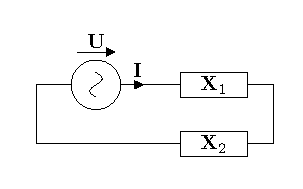
\includegraphics[width=.4\textwidth]{philipCircuits2.pdf}\end{center}
    \only<1>{\begin{align*}
        Z &= \mathbf{X}_1 + \mathbf{X}_2
    \end{align*}}
    % now do smth with that
\end{frame}

\begin{frame}
    \begin{center}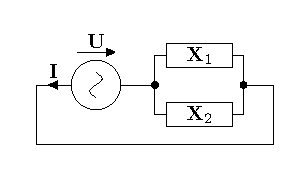
\includegraphics[width=.4\textwidth]{philipCircuits1.pdf}\end{center}
    \only<1>{\begin{align*}
        Z &= \mathbf{X}_1 \parallel \mathbf{X}_2 
        = \frac{1}{\frac{1}{\mathbf{X}_1}+  \frac{1}{\mathbf{X}_2}}
    \end{align*}}
    \only<2-3>{\begin{align*}
        \frac{1}{\mathbf{Z}} \coloneqq \frac{1}{a+b\mathbf{i}} 
        \visible<3>{
            = \frac{a-b\mathbf{i}}{(a+b\mathbf{i})\cdot(a-b\mathbf{i})} 
            = \frac{a-b\mathbf{i}}{a^2+b^2}
            = \frac{1}{r^2} \cdot (a-b\mathbf{i})
        }
    \end{align*}}
    % now do smth with that
\end{frame}

% \begin{frame}
%     % Here be RCL Schwingkreise.
% \end{frame}

% \begin{frame}
%     % Here be Erklärung, dass das alles im komplexen Raum is. 
% \end{frame}

% \begin{frame}
%     % Here be FT ausblick
% \end{frame}


